\documentclass[10pt,a4paper]{article}
\usepackage[utf8]{inputenc}
\usepackage[spanish, mexico]{babel}
\usepackage{listingsutf8}
\usepackage{color}
\usepackage{amsmath}
\usepackage{booktabs}
\usepackage{subcaption}
\usepackage{graphicx}
\usepackage{multicol} 
\usepackage{float}
\usepackage{wasysym}
\definecolor{codegreen}{rgb}{0,0.6,0}
\definecolor{codegray}{rgb}{0.5,0.5,0.5}
\definecolor{codepurple}{rgb}{0.58,0,0.82}
\definecolor{backcolour}{rgb}{0.95,0.95,0.92}
\usepackage[top=2cm,bottom=3cm,left=3cm,right=3cm]{geometry}
\setlength{\parskip}{\baselineskip} 

\begin{document}

\setlength{\unitlength}{1cm}
\thispagestyle{empty}
\begin{picture}(18,4)
\put(0,0.2){
\includegraphics[scale=.2]{UNAM.jpg}}
\put(11.5,0){
\includegraphics[scale=.5]{fc.png}}
\end{picture}
\begin{center}
\textbf{{\LARGE Universidad Nacional Autónoma de México}\\[1cm]
{\LARGE Facultad de Ciencias}}\\[1.8cm]
{\LARGE Práctica 12: Ondas estacionarias en tubos}\\[1.2cm]
\end{center}
\vspace{.7 cm}
\begin{flushleft}{\Large 5 de Noviembre de 2019  }\\[1 cm]
\end{flushleft}
\begin{flushright}{\Large{\underline{\textcolor{black}{López Cruz Ángel Jikmé}}}}\\[0.78cm]
\end{flushright}
\begin{flushright}{\Large{\underline{\textcolor{black}{López Velasco Juan Manuel}}}}\\[0.78cm]

\begin{flushright}{\Large{\underline{\textcolor{black}{Robledo Ibarra Emiliano}}}}\\[1 cm]
\end{flushright}\end{flushright}
\begin{center}
{\Large Profesor: Luis Quintanar Robles }\\[0.4cm]
{\Large Ayudante: Luis Enrique Quintanar Cortés }\\[1 cm]
\end{center}
RESUMEN:
La práctica tuvo como objetivo medir la velocidad del sonido en el aire por medio de un tubo cerrado (abierto en uno de sus lados), utilizando diferentes frecuencias y midiendo la longitud de onda se obtuvo una gráfica con dichos valores, encontrando así, que la pendiente de la gráfica era la velocidad del sonido, el valor de la velocidad del sonido en el aire fue 334 $\pm$ 2 $\frac{m}{s}$ difiriendo 2 $\%$ del valor teórico. Se logró obteniendo una relación entre el inverso de la frecuencia de cada diapasón y la longitud de onda al escuchar el sonido que se generaba al modificar la profundidad.
\normalsize
\newpage


\section{Introducción}

El objetivo de esta práctica fue medir la velocidad del sonido generado al hacer vibrar un diapasón (instrumento metálico en forma de U que al vibrar produce un sonido de frecuencia determinada) en el aire (bajo las condiciones para el mismo en la CDMX). 

Como se vió en la práctica anterior, el sonido se transmite por medio de ondas, las cuales están caracterizadas por diversos parámetros tales como el periodo $T$, amplitud $A$, frecuencia $f$, fase $\phi$ y la longitud de onda $\lambda$. Otra de las características de las ondas es la interferencia, que es el fenómeno en el cual dos ondas se superponen para formar una onda resultante de mayor, menor o igual amplitud. Sabiendo que hay dos tipos de onda: estacionarias y viajeras. Podemos ubicar donde se produce cada una y su como se espera que comporten, debido al sistema que se utilizó se identificó una onda estacionaria.

Una onda estacionaria es el resultado de la interferencia de dos movimientos ondulatorios armónicos de igual amplitud y frecuencia que se propagan en sentidos opuestos a través de un medio. En una onda estacionaria se distinguen los nodos, que son aquellos puntos en que la amplitud es nula, es decir, posiciones donde no hay vibración; los antinodos de la onda estacionaria, que al contrario de los nodos son los puntos en donde la vibración se produce con la máxima amplitud posible.

Se puede considerar que una onda estacionaria no es una onda viajera debido a que tanto los nodos como los antinodos permanecen inmóviles. 

En las ondas estacionarias la distancia entre dos nodos consecutivos (o antinodos) es igual a media longitud de onda. De modo que, como se hizo en la práctica anterior, midiendo tanto la longitud de onda y la frecuencia de la misma se puede entonces medir la velocidad de propagación de la onda (en este caso, las ondas que interfieren para generar el patrón estacionario) en el medio en el cual se estén realizando las mediciones. 

La relación anterior está dada por la siguiente ecuación, 

\begin{equation}
	v = \lambda f
\end{equation}

De manera análoga a la práctica anterior es posible conocer la velocidad de la onda mediante los datos relacionando el inverso de la frecuencia con la longitud de onda:

\begin{equation}
    \lambda = \frac{1}{f}v
\end{equation}

Cabe destacar que se usaron instrumentos sin incertidumbre (diapasones) de los cuales no fue posible obtener una incertidumbre asociada por lo que se utilizaron datos fijos para dichas frecuencias, esto limita de cierta manera al experimento ya que no es posible afirmar con rigurosidad que cada frecuencia utilizada sea la que el instrumento propone, de manera que sabiendo que el material usado pierde sus propiedades se desconoce que tan lejana sea la frecuencia real emitida por el diapasón. De esta forma los resultados son limitados a los instrumentos particulares utilizados.

\newpage
\section{Procedimiento.}
Para poder medir la velocidad del sonido en una onda estacionaria fue necesario poder contener a esta dentro de un recipiente el cual pudiese variar sus dimensiones de profundidad, de forma que al variar dichas dimensiones se escuchasen variaciones en la amplitud de la onda y mientras se variaba la profundidad, se conocía la magnitud de este cambio.

Se consiguió un recipiente lo suficientemente largo como para medir longitudes onda para frecuencias grandes y con una abertura al fondo para poderlo drenar, luego se le adhirió una cinta métrica a su extremo superior  (parte abierta del recipiente). Listo el recipiente se llenó completamente de agua cerrando el orificio que lo drenaba. Se tomó el cuidado de colocar una tina en el recipiente por si ocurrían imprevistos tales como derrames de agua.

Listo el recipiente con el cual se midió y sus complementos, se comenzó a medir las longitudes, se eligieron seis frecuencias para las cuales se midió su longitud de onda: 288 Hz, 341.3 Hz, 384 Hz, 426.7 Hz, 500 Hz y 4000 Hz. Con sus respectivos diapasones se les hizo sonar golpeándolos con un tubo con recubrimiento plástico y posteriormente dejándolo sonar en la parte abierta del recipiente para poder así bajar el nivel del agua y escuchar la onda sonora generada por este efecto. Se hicieron dos mediciones para todas las ondas distintas de 4000 Hz, primero se buscó el primer máximo de la onda y se registró para luego encontrar un segundo máximo y se registró de nuevo, a estas dos mediciones se sumaron y posteriormente se le asoció la incertidumbre de su suma ($\pm0.1$). En el caso especial del diapasón de 4000 Hz se hizo su medición completa, es decir se midió sólo una vez (por repetición) debido a su dificultad de determinar su longitud de onda, fue el que más repeticiones tuvo. Para cada diapasón se le realizaron varias mediciones las cuales sirvieron para determinar tanto la longitud de onda como la reproducibilidad.

\begin{figure}[H]
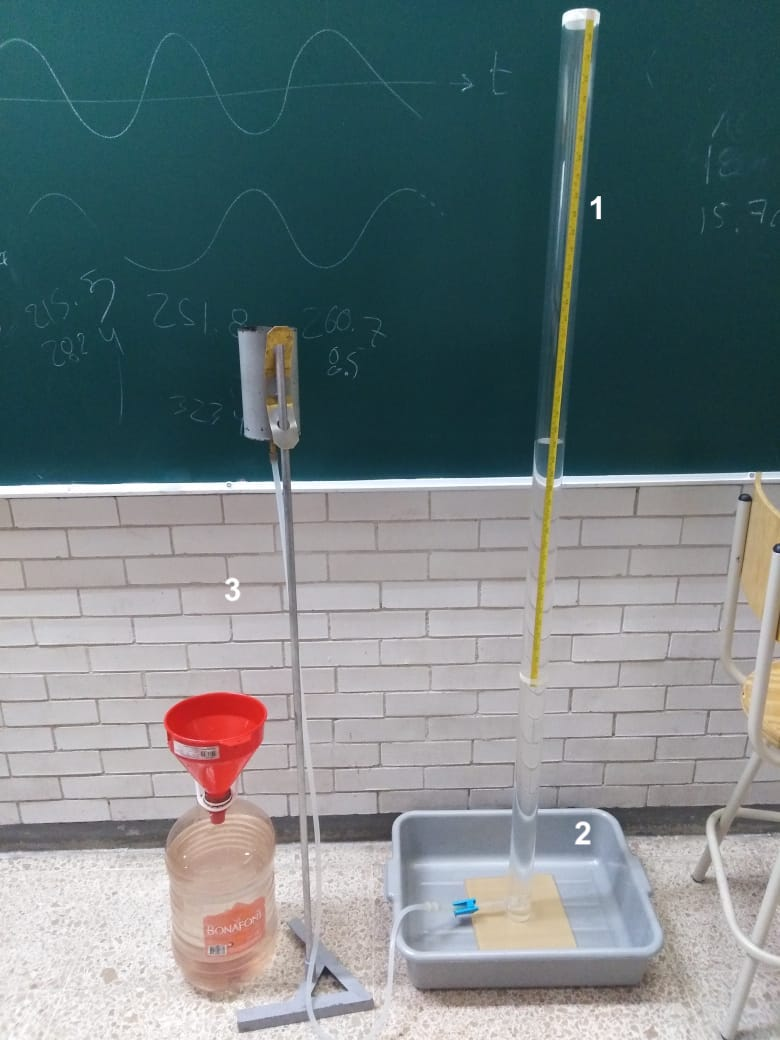
\includegraphics[scale=0.3]{esquema.jpeg}
\centering
\caption{Diseño experimental: 1. Contenedor con cinta. 2. Tina. 3. Contenedores de agua. }
\end{figure}









\section{Resultados}
Se anexan los resultados para cada diapasón en las siguientes tablas.


\begin{table}[H]
    \centering
\begin{minipage}[t]{0.48\linewidth}\centering
\caption{Diapasón de 500 Hz}
\begin{tabular}{ c c }
\toprule
500 Hz   \\
\midrule
Longitud de onda ($\lambda$) [cm]     \\
64.6$\pm0.1$      \\
66.9$\pm0.1$     \\
67.5$\pm0.1$     \\
67.0$\pm0.1$     \\
66.7$\pm0.1$     \\
67.1$\pm0.1$     \\
67.2$\pm0.1$     \\
\bottomrule
\end{tabular}
\end{minipage}\hfill%
\begin{minipage}[t]{0.48\linewidth}\centering
\caption{Diapasón de 384 Hz}
\label{tab:The parameters 2 }
\begin{tabular}{ c c }
\toprule
384 Hz   \\
\midrule
Longitud de onda ($\lambda$) [cm]     \\
88.0$\pm0.1$     \\
88.0$\pm0.1$     \\
87.8$\pm0.1$     \\
87.9$\pm0.1$     \\
86.8$\pm0.1$     \\
88.3$\pm0.1$     \\
88.0$\pm0.1$     \\
\bottomrule
\end{tabular}
\end{minipage}
\end{table}

\begin{table}[H]
    \centering
\begin{minipage}[t]{0.48\linewidth}\centering
\caption{Diapasón de 288 Hz}
\begin{tabular}{ c c }
\toprule
288 Hz   \\
\midrule
Longitud de onda ($\lambda$) [cm]     \\
116.2$\pm0.1$     \\
116.2$\pm0.1$     \\
116.0$\pm0.1$     \\
116.4$\pm0.1$     \\
116.0$\pm0.1$     \\
\bottomrule
\end{tabular}
\end{minipage}\hfill%
\begin{minipage}[t]{0.48\linewidth}\centering
\caption{Diapasón de 426.7 Hz}
\label{tab:The parameters 2 }
\begin{tabular}{ c c }
\toprule
426.7 Hz   \\
\midrule
Longitud de onda ($\lambda$) [cm]     \\
78.2$\pm0.1$     \\
78.5$\pm0.1$     \\
78.0$\pm0.1$     \\
78.4$\pm0.1$     \\
78.3$\pm0.1$     \\
\bottomrule
\end{tabular}
\end{minipage}
\end{table}


\begin{table}[H]
    \centering
\begin{minipage}[t]{0.48\linewidth}\centering
\caption{Diapasón de 4000 Hz}
\begin{tabular}{ c c }
\toprule
4000 Hz   \\
\midrule
Longitud de onda ($\lambda$) [cm]     \\
8.70$\pm0.05$     \\
8.50$\pm0.05$     \\
9.70$\pm0.05$     \\
9.20$\pm0.05$     \\
8.50$\pm0.05$     \\
9.20$\pm0.05$     \\
11.70$\pm0.05$     \\
7.00$\pm0.05$     \\
6.80$\pm0.05$     \\
\bottomrule
\end{tabular}
\end{minipage}\hfill%
\begin{minipage}[t]{0.48\linewidth}\centering
\caption{Diapasón de 341.3 Hz}
\label{tab:The parameters 2 }
\begin{tabular}{ c c }
\toprule
341.3 Hz \\
\midrule
Longitud de onda ($\lambda$) [cm]     \\
98.0$\pm0.1$     \\
98.4$\pm0.1$     \\
98.4$\pm0.1$     \\
98.3$\pm0.1$     \\
98.4$\pm0.1$     \\
\bottomrule
\end{tabular}
\end{minipage}
\end{table}
 
Una vez obtenidas las longitudes de onda se promediaron para poder obtener un solo dato que tratar a cada frecuencia y con esta longitud de onda y la frecuencia asociada se graficó el inverso de la frecuencia contra la longitud para poder ajustarle una recta que como anteriormente se hizo tendría como pendiente la velocidad de dicha onda. 

% Table generated by Excel2LaTeX from sheet 'Sheet1'
\begin{table}[H]
  \centering
    \begin{tabular}{|c|c|c|} \hline
    Frecuencia [Hz] & Longitud de onda [m] & Inverso de la frecuencia ($\frac{1}{f}$) [Hz] \\ \hline
    288 Hz & 1.162$\pm0.002$ & 0.0034722 \\ \hline
    341.3 Hz & 0.983$\pm0.003$ & 0.0029300 \\ \hline
    384 Hz & 0.88$\pm0.01$ & 0.0026042 \\ \hline
    426.7 Hz & 0.783$\pm0.003$ & 0.0023436 \\ \hline
    500 Hz & 0.67$\pm0.02$ & 0.0020000 \\ \hline
    4000 Hz & 0.09$\pm0.03$ & 0.0002500 \\ \hline
    \end{tabular}%
  \caption{Datos a graficar, obtenidos del diapasón y del promedio de la medición.}
\end{table}%
 
 Y al graficar los datos con un ajuste se obtiene:
 
 \begin{figure}[H]
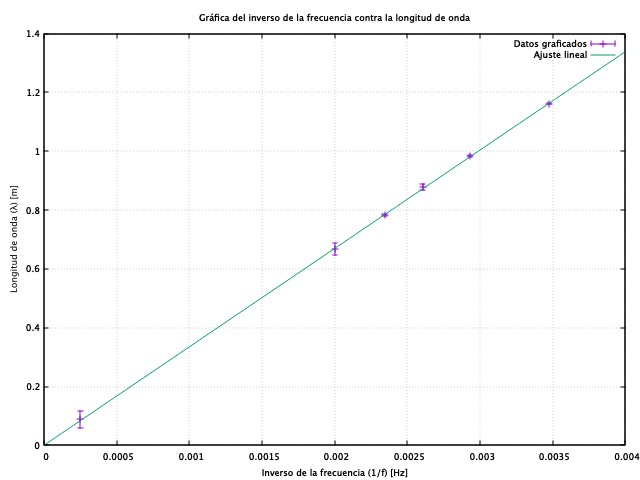
\includegraphics[scale=0.5]{grafica.jpeg}
\centering
\caption{Ajustes de rectas hechos a los datos del aire con recta de (334 $\pm$ 2)X + (0.000 $\pm$ 0.005)}
\end{figure}

Con la pendiente de $m = (334\pm2)$.

\section{Análisis de datos}
Los valores obtenidos en la longitud de onda en las diferentes frecuencias, no fueron reproducibles, por tal razón fueron medidos repetida veces aunque  sus valores fueron cercanos entre sí.

La velocidad del sonido teórico a una temperatura de 20 grados centígrados es de 344 $\frac{m}{s}$, el valor obtenido en la medición de la velocidad del sonido fue de 334 $\pm$ 2 $\frac{m}{s}$ el valor teórico no se encuentra dentro del intervalo de incertidumbre, pero el valor central de la medida es 3 $\%$ menor al valor teórico.

El valor del coeficiente de determinación de la relación entre el inverso de la frecuencia y la longitud de onda fue de 0.9999, lo que nos indica que la velocidad obtenida fue bastante precisa.

\section{Conclusiones}

\begin{itemize}
    \item La velocidad del sonido encontrado fue de 334 $\pm$ 2 $\frac{m}{s}$ siendo 2 $\%$ menor al valor teórico.
    \item Gracias al valor del coeficiente de determinación de la relación se puede observar que prácticamente es una recta el comportamiento que se está midiendo por lo que la relación entre las variables $\frac{1}{f}$ y $\lambda$ es lineal.
    \end{itemize}
El sonido es una onda longitudinal que depende del medio dónde se propague, es decir el sonido es una serie de compresiones y descompresiones en el medio, lo que provoca áreas de máxima y mínima presión (o alta densidad), en la práctica se mostró como encontrar el valor de la velocidad del sonido por medio de un contenedor el cual como era un tubo cerrado (abierto sólo en un
extremo), las frecuencias de modo normal son los múltiplos
impares de la rapidez del sonido dividida entre 4 veces la longitud (desde la parte abierta hasta el máximo medido), es decir en la práctica se midió el antinodo hasta el segundo máximo, lo cual para conocer la longitud de onda $\lambda= \frac{4}{3}*L$ siendo L la longitud medida,  a comparación con la práctica 11 que se usó para medir la velocidad del sonido un tubo que formaba dos nodos. 

Sabiendo que el ajuste resultó muy bueno y además de ser muy cercano al valor esperado, nos es posible no sólo confiar en el resultado obtenido sino que podemos extraer más información; se utilizó que los diapasones contaban con frecuencias sin incertidumbre, es decir datos fijos, aunque sabemos que no es posible obtener dicho instrumento sin incertidumbre podemos observar que las mediciones que se obtuvieron son lo suficientemente próximas a las cuales se esperarían por lo cual podemos decir que los instrumentos generan una frecuencia acorde a la que mencionan. 

Por último, se contó con un problema notorio acerca de la medición de una frecuencia, en concreto la de 4000 Hz ya que se puede observar una incertidumbre del 30\% para su longitud de onda, resultó extremadamente difícil la medición de dicha longitud debido a la velocidad de drenado de agua y la proximidad de cada elemento en la onda (nodos y antinodos), por lo que se recomienda no tomar frecuencias tan altas que resulten en situaciones difíciles de controlar.


\begin{thebibliography}{a}

\bibitem{pradery} \textsc{A., J., Barbero} (2007). \textit{Ondas Estacionarias}. Recuperado el 8 de Noviembre del 2019, de:  https://previa.uclm.es/profesorado/ajbarbero/CursoAB2007/OndasEstacionarias06.pdf

\bibitem{Baz} \textsc{Freedman, Young }(2001). 
\textit{Sonido y oido: Velocidad del sonido en fluidos. En Física Universitaria volúmen 1}. Recuperado el 9 de Noviembre del 2019.


\end{thebibliography}

\end{document}
